
You can insert queries into your file (despite the Coq IDE giving a warning), or you can use the query pane. 
The results of a query will appear in the messages pane.
There are many types of queries, including the ones described below. 
See file ``Queries.v" to follow along.

\subsection{Query Pane} \label{query_pane}
To open the query pane, either press F1 or go to the View tab, then down to the Query Pane option. 
The query pane is more convenient when you're in the middle of a proof but need to look up something; 
however, when doing multiple queries from the query pane, the results will show up in the messages tab without clearing the results of previous queries.

~\\
\begin{minipage}{\textwidth}
\centered{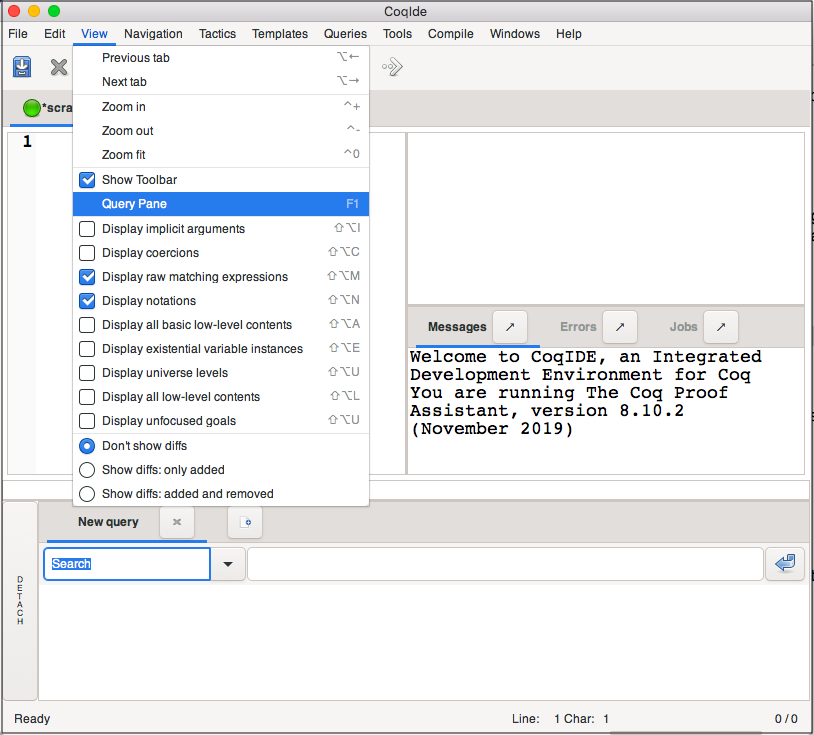
\includegraphics[width=15cm]
        {CoqScreenshots/query_pane_10.png}}
\end{minipage}

\noindent
You can detach the query pane into its own window by pressing the Detach button along the lefthand side of the query pane.
This is particularly useful when you are doing proofs and need to search to find the correct property to use 
(Coq has tons of properties defined in its libraries).




\newpage
\subsection{Search} \label{search}
Searches the environment for the given name, then displays the name and type of all objects that contains the name. 
This is useful to find out information about libraries and pre-defined theorems. 

\begin{code}
	Search plus.
\end{code}
\begin{msg}
	plus\_O\_n: forall n : nat, 0 + n = n	\\
	plus\_n\_O: forall n : nat, n = n + 0	\\
	plus\_n\_Sm: forall n m : nat, S (n + m) = n + S m	\\
	plus\_Sn\_m: forall n m : nat, S n + m = S (n + m)	\\
	mult\_n\_Sm: forall n m : nat, n * m + n = n * S m		\\
	f\_equal2\_plus: forall x1 y1 x2 y2 : nat, x1 = y1 $->$ x2 = y2 $->$ x1 + x2 = y1 + y2	\\
	nat\_rect\_plus:	\\ \-\ \quad
	  forall (n m : nat) (A : Type) (f : A $->$ A) (x : A),	\\ \-\ \quad
	  nat\_rect (fun \_ : nat $=>$ A) x (fun \_ : nat $=>$ f) (n + m) =	\\ \-\ \quad
	  nat\_rect (fun \_ : nat $=>$ A) (nat\_rect (fun \_ : nat $=>$ A) x (fun \_ : nat $=>$ f) m)	
	  \\ \-\ \qquad
	    (fun \_ : nat $=>$ f) n
\end{msg}

\noindent 
Searching multiple names obtains more specific results. 

\hspace{-1cm}
\begin{tabular}{p{8cm} p{8cm}}
\begin{code}
	Search plus 0. \\
\end{code}&
\begin{msg}
	plus\_O\_n: forall n : nat, 0 + n = n	\\
	plus\_n\_O: forall n : nat, n = n + 0
\end{msg}
\end{tabular}

\noindent 
If you haven't loaded the library corresponding to what you are searching, you will get fewer results; you may need to load the library if you can't find what you need. For example,
\begin{code}
	Search plus Nat.odd.
\end{code}
yields no results when the Arith library hasn't been added, but once we have imported the library we receive five results.
\begin{code}
	\cmd{Require Import} Arith. 	\\
	Search plus Nat.odd.
\end{code}
\begin{msg}
	Nat.odd\_add\_even: forall n m : nat, Nat.Even m $->$ Nat.odd (n + m) = Nat.odd n	\\
	Nat.odd\_add: forall n m : nat, Nat.odd (n + m) = xorb (Nat.odd n) (Nat.odd m)		\\
	Nat.odd\_add\_mul\_even: forall n m p : nat, Nat.Even m $->$ Nat.odd (n + m * p) = Nat.odd n	\\
	Nat.odd\_add\_mul\_2: forall n m : nat, Nat.odd (n + 2 * m) = Nat.odd n	\\
	Nat.div2\_odd: forall a : nat, a = 2 * Nat.div2 a + Nat.b2n (Nat.odd a)
\end{msg}

\noindent
You can also search for patterns: enclose the pattern in parentheses, and use an underscore for arbitrary terms.
\begin{code}
	Search $(\sim \_ <-> \_\ )$.
\end{code}
\begin{msg}
	neg\_false: forall A : Prop, $\sim$ A $<->$ (A $<->$ False)		\\
	not\_iff\_compat: forall A B : Prop, A $<->$ B $->$ $\sim$ A $<->$ $\sim$ B
\end{msg}




\subsection{SearchRewrite} \label{search_rewrite}
Searches the environment for a statement with an equality that contains the given pattern on at least one side.
\begin{code}
	SearchRewrite $(\_ * \_\ / \_\ )$.
\end{code}
\begin{msg}
	Nat.div\_mul: forall a b : nat, b $<>$ 0 $->$ a * b / b = a	\\
	Nat.divide\_div\_mul\_exact: 
 		forall a b c : nat, b $<>$ 0 $->$ Nat.divide b a $->$ c * a / b = c * (a / b)	\\
	Nat.div\_mul\_cancel\_l: forall a b c : nat, b $<>$ 0 $->$ c $<>$ 0 $->$ c * a / (c * b) = a / b	\\
	Nat.div\_mul\_cancel\_r: forall a b c : nat, b $<>$ 0 $->$ c $<>$ 0 $->$ a * c / (b * c) = a / b	\\
	Nat.lcm\_equiv1:
  		forall a b : nat, Nat.gcd a b $<>$ 0 $->$ a * (b / Nat.gcd a b) = a * b / Nat.gcd a b	\\
	Nat.lcm\_equiv2:
  		forall a b : nat, Nat.gcd a b $<>$ 0 $->$ a / Nat.gcd a b * b = a * b / Nat.gcd a b
\end{msg}





\subsection{Check} \label{check}
Displays the type of the given term.

\hspace{-1cm}
\begin{tabular}{p{8cm} p{8cm}}
	\begin{code} 	\cmd{Check} 0. 				\end{code}	%1
	\begin{code}	\cmd{Check} nat.				\end{code}	%2
	\begin{code}	\cmd{Check} plus.				\end{code}	%3
	&
	\begin{msg} 	0  : nat 						\end{msg}		%1
	\begin{msg}	nat : Set						\end{msg}		%2
	\begin{msg}	Nat.add : nat $->$ nat $->$ nat		\end{msg}		%3
\end{tabular}



\subsection{About} \label{about}
Displays information about the object with the given name 
(i.e. its kind, type, arguments).

\hspace{-1cm}
\begin{tabular}{p{8cm} p{8cm}}
	\begin{code} 	
		\cmd{About} plus. 	\\		
	\end{code}	
	&
	\begin{msg} 	
		Notation plus := Init.Nat.add	\\
		Expands to: Notation Coq.Init.Peano.plus
	\end{msg}
\end{tabular}





\subsection{Locate} \label{locate}
Displays the full name of the given term and what Coq module it is defined in.

\hspace{-1cm}
\begin{tabular}{p{8cm} p{8cm}}
	\begin{code} 	Locate plus. 					\end{code}	%1
	\begin{code} 	Locate nat. 					\end{code}	%2
	&
	\begin{msg} 	Notation Coq.Init.Peano.plus		\end{msg}		%1
	\begin{msg} 	Inductive Coq.Init.Datatypes.nat	\end{msg}		%2
\end{tabular}




\subsection{Print} \label{print}
Displays information about the given name.

\hspace{-1cm}
\begin{tabular}{p{8cm} p{8cm}}
	\begin{code} 	\cmd{Print} plus. 				\end{code}
	&
	\begin{msg} 	Notation plus := Init.Nat.add			\end{msg}	
\end{tabular}

\noindent
It is possible to see what is currently loaded and imported in the environment with the following:

\hspace{-1cm}
\begin{tabular}{p{8cm} p{8cm}}
	\begin{code} 	\cmd{Print} Libraries. \\ \\ \\ \\ \\ \\ \\ \\ \\ \\ \\ \\ \end{code}
	&
	\begin{msg} 	
		Loaded and imported library files: 	\\ \-\ \quad
		  Coq.Init.Notations				\\ \-\ \quad
		  Coq.Init.Logic					\\ \-\ \quad
		  Coq.Init.Logic\_Type			\\ \-\ \quad
		  Coq.Init.Datatypes				\\ \-\ \quad
		  Coq.Init.Specif				\\ \-\ \quad
		  Coq.Init.Peano				\\ \-\ \quad
		  Coq.Init.Wf					\\ \-\ \quad
		  Coq.Init.Tactics				\\ \-\ \quad
		  Coq.Init.Tauto					\\ \-\ \quad
		  Coq.Init.Prelude				\\
		Loaded and not imported library files: \\ \-\ \quad
		  Coq.Init.Nat
	\end{msg}	
\end{tabular}





\subsection{Print Assumptions} \label{print_assumptions}
Displays all assumptions depended upon by the object of the given name.

\hspace{-1cm}
\begin{tabular}{p{8cm} p{8cm}}
	\begin{code} 	\cmd{Print} Assumptions plus. 			\end{code}
	&
	\begin{msg} 	Closed under the global context		\end{msg}	
\end{tabular}







%\subsection{} \label{}




